\documentclass[a4paper]{article}

%use the english line for english reports
%usepackage[english]{babel}
\usepackage[portuguese]{babel}
\usepackage[utf8x]{inputenc}
\usepackage{indentfirst}
\usepackage{graphicx}
\usepackage{verbatim}
\usepackage[top=2.5cm, bottom=3cm, left=2.5cm, right=2.5cm]{geometry}

\begin{document}

%\setlength{\textwidth}{16cm}
%\setlength{\textheight}{22cm}

\title{\Huge\textbf{Dominup em Prolog}\linebreak\linebreak\linebreak
\Large\textbf{Relatório Intercalar}\linebreak\linebreak
\linebreak\linebreak

\includegraphics[scale=0.1]{feup-logo.png}\linebreak\linebreak
\linebreak\linebreak
\Large{Mestrado Integrado em Engenharia Informática e Computação} \linebreak\linebreak
\Large{Programação em Lógica}\linebreak
}

\author{\textbf{Dominup4:}\\
Ângela Filipa Pereira Cardoso - up200204375 \\
Nuno Miguel Rainho Valente - up200204376 \\
\linebreak\linebreak \\
 \\ Faculdade de Engenharia da Universidade do Porto \\ Rua Roberto Frias, s\/n, 4200-465 Porto, Portugal \linebreak\linebreak\linebreak
\linebreak\linebreak\vspace{1cm}}

\maketitle
\thispagestyle{empty}

%************************************************************************************************
%************************************************************************************************

\newpage

%Todas as figuras devem ser referidas no texto. %\ref{fig:codigoFigura}
%
%%Exemplo de código para inserção de figuras
%%\begin{figure}[htbp]
%%\begin{center}
%%escolher entre uma das seguintes três linhas:
%%\includegraphics[height=20cm,width=15cm]{path relativo da imagem}
%%\includegraphics[scale=0.5]{path relativo da imagem}
%%\includegraphics{path relativo da imagem}
%%\caption{legenda da figura}
%%\label{fig:codigoFigura}
%%\end{center}
%%\end{figure}
%
%
%\textit{Para escrever em itálico}
%\textbf{Para escrever em negrito}
%Para escrever em letra normal
%``Para escrever texto entre aspas''
%
%Para fazer parágrafo, deixar uma linha em branco.
%
%Como fazer bullet points:
%\begin{itemize}
	%\item Item1
	%\item Item2
%\end{itemize}
%
%Como enumerar itens:
%\begin{enumerate}
	%\item Item 1
	%\item Item 2
%\end{enumerate}
%
%\begin{quote}``Isto é uma citação''\end{quote}


%%%%%%%%%%%%%%%%%%%%%%%%%%
\section{O Jogo Dominup}

Dominup é uma variação do jogo Dominó para 2 a 4 jogadores, em que, tal como o nome sugere, é possível colocar peças em cima de outras.

No típico Dominó existem 28 peças duplas numeradas de 0 a 6, à semelhança das faces de um dado. Já no Dominup há 36 peças duplas numeradas de 0 a 7, usando códigos binários: o ponto no centro representa 1, o circulo pequeno representa 2 e o circulo grande representa 4, como se pode ver na figura~\ref{piece}. Este desenho das peças, juntamente com as regras do Dominup e de dois outros jogos, foram criadas por Néstor Romeral Andrés em 2014, sendo o conjunto publicado por nestorgames\footnote[1]{http://www.nestorgames.com}.

\begin{figure}[htbp]
\begin{center}

\includegraphics[scale=0.5]{piece.jpg}
\caption{Exemplo da peça $3 \cdot 6$.}
\label{piece}
\end{center}
\end{figure}

Existem dois tipos de colocação de peças no Dominup:
\begin{itemize}
	\item subir - a peça é colocada em cima de duas peças adjacentes que estejam ao mesmo nível, de forma a que os números da peça colocada sejam iguais aos que ficam por baixo (um em cada peça de suporte), tal como mostra a figura~\ref{climb}.
	\item expandir - a peça é colocada na superfície de jogo, de forma a que fique adjacente e ortogonal a pelo menos uma peça já colocada, como, por exemplo, as duas peças já colocadas na figura~\ref{climb}.
\end{itemize}

\begin{figure}[htbp]
\begin{center}
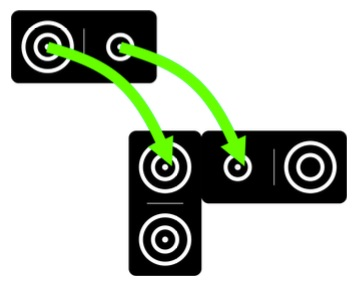
\includegraphics[scale=0.6]{climb.jpg}
\caption{Exemplo de um posicionamento a subir válido.}
\label{climb}
\end{center}
\end{figure}

Tal como no Dominó, as regras são relativamente simples. Começa-se por distribuir as peças aleatoriamente e de forma equilibrada pelos jogadores, mantendo a face voltada para baixo. 

O jogador com o duplo 7 inicia o jogo, colocando essa peça no centro da superfície de jogo e determinando a ordem dos restantes jogadores, que é dada pelo sentido contrário ao ponteiro dos relógios. 

Começando no segundo, cada jogador, na sua vez, realiza ambos os passos seguintes:
\begin{enumerate}
	\item Enquanto for possível, coloca peças a subir, podendo escolher a ordem em que o faz;
	\item Se ainda tiver alguma peça, coloca-a a expandir.
\end{enumerate}

Se, no final da sua vez, o jogador ficar sem peças, é declarado vencedor e o jogo termina. Alternativamente, os restantes jogadores podem continuar, de forma a determinar o segundo, terceiro e quarto lugares.

Na figura~\ref{example} pode ser observado um possível jogo de Dominup a decorrer.

\begin{figure}[htbp]
\begin{center}
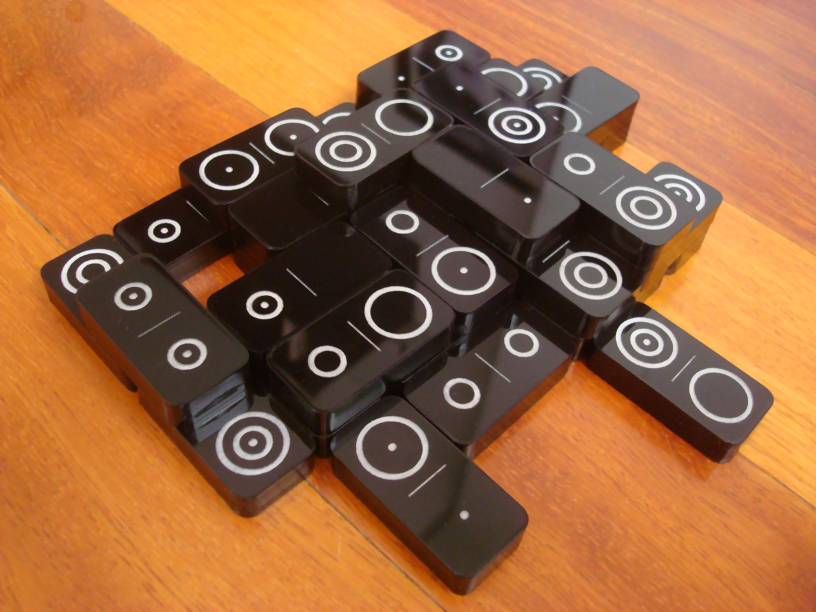
\includegraphics[scale=0.4]{example.jpg}
\caption{Exemplo de um jogo de Dominup.}
\label{example}
\end{center}
\end{figure}


%Descrever detalhadamente o jogo, a sua história e, principalmente, as suas regras.
%Devem ser incluidas imagens apropriadas para explicar o funcionamento do jogo.
%Devem ser incluidas as fontes de informação (e.g. URLs em rodapé).


%%%%%%%%%%%%%%%%%%%%%%%%%%
\section{Representação do Estado do Jogo}

O tabuleiro de jogo no Dominup é um quadriculado, cujo tamanho não deve limitar o posicionamento de peças a expandir. Uma vez que expansões sucessivas têm que ser feitas ortogonalmente, uma linha expansiva numa só direção ocupa $2 + 1 + 2 + 1 + \cdots$ quadrículas, assumindo que a primeira peça está colocada horizontalmente. Ao todo temos 36 peças, por isso seriam necessárias $2 * 18 + 18 = 54$ quadrículas para acomodar uma tal linha de expansão. Dado que a primeira peça é colocada no centro do tabuleiro, se a expansão fosse feita sempre no mesmo sentido, poderíamos ter que considerar um tabuleiro com 108 quadrículas de lado.

Uma análise mais cuidada das regras do jogo revela que as peças são preferencialmente colocadas a subir. De facto, em cada vez, um jogador coloca tantas peças a subir quanto possível e no máximo uma peça a expandir. Além disso, em geral não será boa estratégia para nenhum dos jogadores expandir sempre no mesmo sentido. Tendo em consideração as limitações de um computador, quer em termos de capacidade de processamento, quer em termos de tamanho do ecrã, decidimos considerar um tabuleiro quadriculado de lado 24. Desta forma, é possível colocar pelo menos 8 peças em cada um dos 4 sentidos a partir do centro do tabuleiro. Eventualmente, com a experiência, podemos decidir reduzir ou aumentar este tamanho. O ideal é que o tabuleiro nunca limite as jogadas, mantendo-se tão pequeno quanto possível para facilitar o processamento.

Sendo assim, o tabuleiro em Prolog é representado por uma lista \verb|board| de 24 linhas do tabuleiro. Por sua vez, cada linha é uma lista de 24 elementos, um para cada quadrícula. Cada elemento de uma linha é um termo complexo \verb|halfPiece(Number, Level, Cardinal)| representando a meia peça de dominó lá colocada, com o seguinte significado:
\begin{itemize}
	\item \verb|Number| é o número da meia peça;
	\item \verb|Level| é o nível do tabuleiro em que a peça está colocada, 1 se for colocada em cima do tabuleiro, 2 se for colocada em cima dessa, etc;
	\item \verb|Cardinal| é o ponto cardeal que indica a posição da outra metade da peça.
\end{itemize}
Assim, numa quadrícula vazia temos \verb|halfPiece(_, _, _)|. Quando é colocado o dominó duplo 7, teremos \verb|halfPiece(7, 1, e)| e \verb|halfPiece(7, 1, o)| em duas quadrículas adjacentes. Numa fase mais avançada pode ser colocado o dominó $2 \cdot 6$ no nível 3 na vertical com \verb|halfPiece(2, 3, n)| e \verb|halfPiece(6, 3, s)|.

Além do tabuleiro, o estado de jogo contém as peças de cada jogador. Dado que apenas consideramos dois jogadores nesta implementação, teremos as listas \verb|set1| e \verb|set2| com as peças dos jogadores 1 e 2, respetivamente. À medida que vão sendo colocadas no tabuleiro, as peças são retiradas destas listas. Cada peça é representada pelo termo complexo \verb|piece(Number1, Number2)|, por exemplo, \verb|piece(2, 6)|, convencionando-se que o primeiro número é sempre menor ou igual ao segundo.

Finalmente, o estado de jogo terá indicação de qual é o próximo jogador a jogar na variável \verb|playerTurn|, que pode ser 1 ou 2. Assim, o estado de jogo é representado por \verb|state(set1, set2, playerTurn, board)|.

Um possível estado inicial, já com as peças distribuídas aleatoriamente pelos jogadores, é dado por:
\begin{itemize}
\item 
\verb|set1([piece(0, 1), piece(0, 3), piece(0, 4), piece(0, 6), piece(1, 1),|\linebreak
\verb|      piece(1, 2), piece(1, 4), piece(1, 5), piece(1, 7), piece(2, 2),|\linebreak
\verb|      piece(2, 3), piece(2, 6), piece(3, 3), piece(3, 7), piece(4, 5),|\linebreak
\verb|      piece(5, 6), piece(6, 7), piece(7, 7)]);|
\item
\verb|set2([piece(0, 0), piece(0, 2), piece(0, 5), piece(0, 7), piece(1, 3),|\linebreak
\verb|      piece(1, 6), piece(2, 4), piece(2, 5), piece(2, 7), piece(3, 4),|\linebreak
\verb|      piece(3, 5), piece(3, 6), piece(4, 4), piece(4, 6), piece(4, 7),|\linebreak
\verb|      piece(5, 5), piece(5, 7), piece(6, 6)]);|
\item \verb|playerTurn(1);|	
\item 
\verb|board([[halfPiece(_, _, _), halfPiece(_, _, _), ..., halfPiece(_, _, _)], ...,|\linebreak
\verb|       [halfPiece(_, _, _), halfPiece(_, _, _), ..., halfPiece(_, _, _)]]).|
\end{itemize}

\begin{figure}[htbp]
\begin{center}
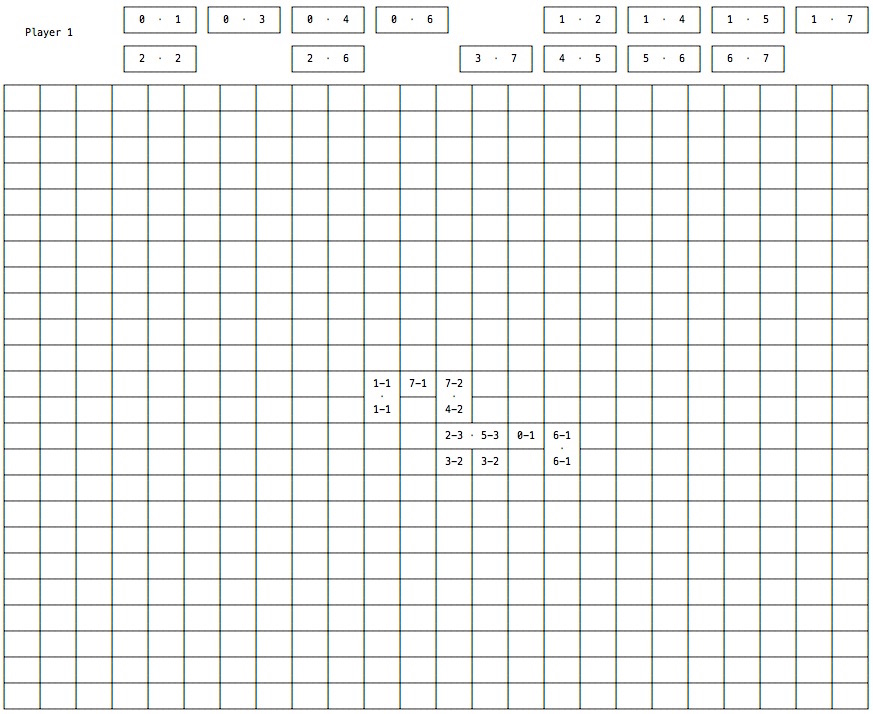
\includegraphics[scale=0.44]{intermediate.jpg}
\caption{Estado intermédio do jogo.}
\label{intermediate}
\end{center}
\end{figure}

Após algumas jogadas, podemos chegar ao estado ilustrado pela Figura~\ref{intermediate}. Em cima estão as peças do jogador 1, dado que esse é o próximo a jogar. Em baixo está o tabuleiro com as peças que contém até então. Cada meia peça colocada no tabuleiro tem do lado esquerdo o seu número e do lado direito o nível em que se encontra. Este estado intermédio é dado pelos seguintes termos:

\begin{itemize}
\item 
\verb|set1([piece(0, 1), piece(0, 3), piece(0, 4), piece(0, 6), piece(1, 2),|\linebreak
\verb|      piece(1, 4), piece(1, 5), piece(1, 7), piece(2, 2), piece(2, 6),|\linebreak
\verb|      piece(3, 7), piece(4, 5), piece(5, 6), piece(6, 7)]);|
\item
\verb|set2([piece(0, 0), piece(0, 2), piece(0, 7), piece(1, 3), piece(1, 6),|\linebreak
\verb|      piece(2, 7), piece(3, 4), piece(3, 6), piece(4, 4), piece(4, 6),|\linebreak
\verb|      piece(5, 5), piece(5, 7)]);|
\item \verb|playerTurn(1);|	
\item 
\verb|board([[halfPiece(_, _, _), halfPiece(_, _, _), ..., halfPiece(_, _, _)],|\linebreak
\verb|       ...,|\linebreak
\verb|       [halfPiece(_, _, _), halfPiece(_, _, _), ..., halfPiece(_, _, _)],|\linebreak
\verb|       [..., halfPiece(1, 1, s), halfPiece(7, 1, e), halfPiece(7, 2, s), ...]|\linebreak
\verb|       [..., halfPiece(1, 1, n), halfPiece(_, _, _), halfPiece(4, 2, n), ...]|\linebreak
\verb|       [..., halfPiece(2, 3, e), halfPiece(5, 3, o), halfPiece(0, 1, o),|\linebreak
\verb|       halfPiece(6, 1, s), ...]|\linebreak
\verb|       [..., halfPiece(3, 2, n), halfPiece(3, 2, n), halfPiece(_, _, _),|\linebreak
\verb|       halfPiece(6, 1, n), ...]|\linebreak
\verb|       [halfPiece(_, _, _), halfPiece(_, _, _), ..., halfPiece(_, _, _)],|\linebreak
\verb|       ...,|\linebreak
\verb|       [halfPiece(_, _, _), halfPiece(_, _, _), ..., halfPiece(_, _, _)]]).|\linebreak
\end{itemize}

\begin{figure}[htbp]
\begin{center}
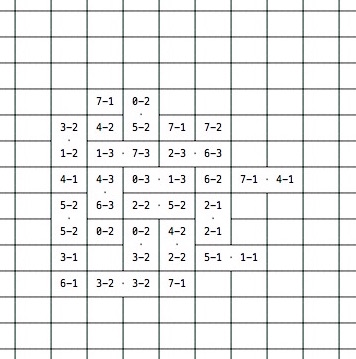
\includegraphics[scale=0.6]{over.jpg}
\caption{Estado final do jogo.}
\label{over}
\end{center}
\end{figure}

Um possível estado final, correspondente ao jogo da Figura~\ref{example}, deverá ter a ilustração da Figura~\ref{over} e, à exceção do tabuleiro, cuja representação é demasiado complexa para traduzir neste relatório, tem os seguintes termos:
\begin{itemize}
\item 
\verb|set1([]);|
\item
\verb|set2([]);|
\item \verb|playerTurn(2);|	
\end{itemize}

%Descrever a forma de representação do estado do tabuleiro (tipicamente uma lista de listas), com exemplificação em Prolog de posições iniciais do jogo, posições intermédias e finais, acompanhadas de imagens ilustrativas.

\begin{figure}[htbp]
\begin{center}
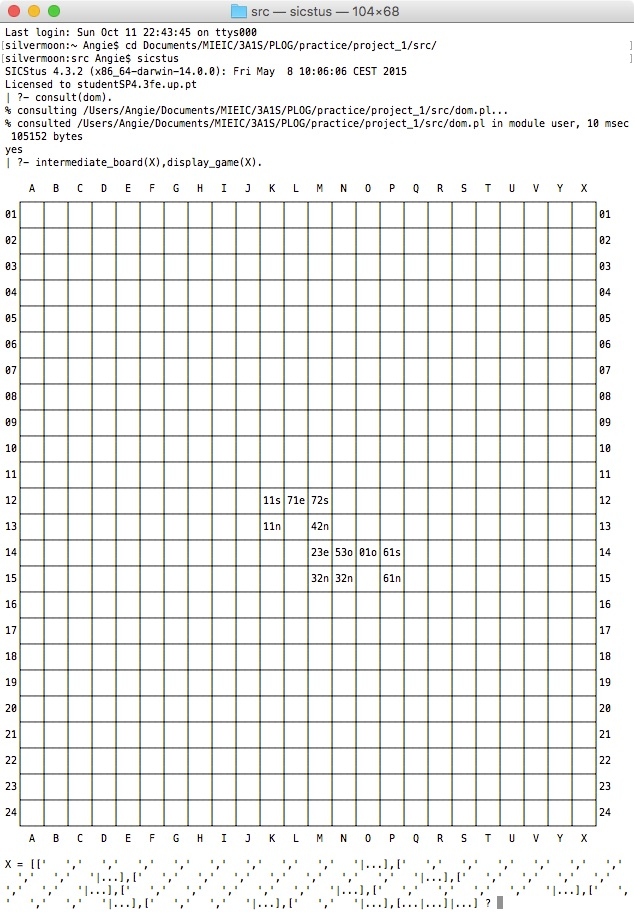
\includegraphics[scale=0.7]{inter_output.jpg}
\caption{Visualização do tabuleiro em Prolog.}
\label{inter_output}
\end{center}
\end{figure}

%%%%%%%%%%%%%%%%%%%%%%%%%%
\section{Visualização do Tabuleiro}

Para visualizar o tabuleiro em modo de texto, começamos por idealizar o formato das Figuras~\ref{intermediate} e~\ref{over}. No entanto, para tal seria necessário desenhar quadrículas diferentes consoante as posições das peças, o que é relativamente complexo de executar. Sendo assim, pelo menos para já, cada quadrícula será sempre desenhada com traços a toda a volta, independentemente da posição das peças. Cada peça é colocada em duas quadrículas adjacentes e a relação entre as duas metades é identificada pelo conteúdo das células. Isto é, o dominó~$2 \cdot 5$ dá origem às células \verb|23e| e \verb|53o|, se for colocado no nível 3 na horizontal com o 2 à esquerda do 5.

Para obter a visualização descrita acima, usamos os seguintes predicados em Prolog:
\begin{itemize}
	\item 
	\begin{verbatim}
		display_game([X|Y]) :- nl, putLetters, nl,
	\end{verbatim}
	\verb|write('  ------------------------------------------'), nl,|
	\begin{verbatim}
		rows(1, [X|Y]), putLetters, nl, nl,!.
	\end{verbatim}
	\item
	\begin{verbatim}
		rows(N, [X|Y]):-putLeftNumbers(N), analyse(X), putRightNumbers(N), nl,
	\end{verbatim}
	\verb|putGrid(N), N1 is N+1, nl, rows(N1, Y).|\linebreak
	\verb|rows(_,[]).|
	\item
	\verb|putLetters:-write('    A   B   C   D   E   F   G   H   I   J   K   ... ').|
	\item
	\verb|putLeftNumbers(N):-((N<10, write(0), write(N), write('|')) ; (write(N), write('|'))).|
	\item
	\verb|putRightNumbers(N):-((N<10, write(0), write(N)) ; (write(N))).|
	\item
	\begin{verbatim}
		putGrid(N):-((N<24, write(' |---|---|---|---|---|---|---|---|---|---|---|'));
	\end{verbatim}
	\verb|write('  ------------------------------------------')) ).|
	\item
	\verb|analyse([]):-!.|
	\begin{verbatim}
		analyse([X|Z]):-print(X),  write('|'), analyse(Z).
	\end{verbatim}
\end{itemize}
De facto, os predicados são ligeiramente diferentes, por o \LaTeX não aceita os caracteres unicode usados para desenhar as quadrículas. De qualquer forma, o resultado está disponível na Figura~\ref{inter_output} cuja configuração é a mesma da Figura~\ref{intermediate}.

%Descrever a forma de visualização do tabuleiro em modo de texto e o(s) predicado(s) Prolog construídos para o efeito.
%Deve ser incluída pelo menos uma imagem correspondente ao output produzido pelo predicado de visualização.

\begin{figure}[ht]
 \begin{minipage}[t]{.5\textwidth}
	\begin{center}
		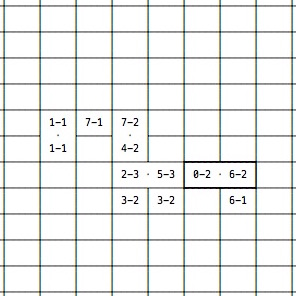
\includegraphics[scale=0.6]{inter_climb.jpg}
		\caption{Movimento a subir.}
		\label{inter_climb}
	\end{center}
 \end{minipage}
 \begin{minipage}[t]{.5\textwidth}
	\begin{center}
		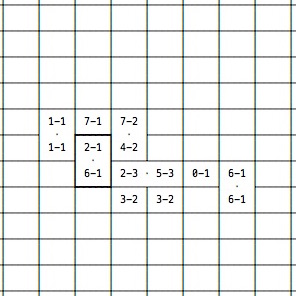
\includegraphics[scale=0.6]{inter_expand.jpg}
		\caption{Movimento a expandir.}
		\label{inter_expand}
	\end{center}
 \end{minipage}
\end{figure}

%%%%%%%%%%%%%%%%%%%%%%%%%%
\section{Movimentos}

De acordo com as regras, na sua vez, um jogador pode realizar vários movimentos, isto é, colocar várias peças no tabuleiro. Mais especificamente, devem ser colocadas todas as peças possíveis a subir (pela ordem que o jogador escolher) e, caso ainda exista, uma peça a expandir. Para realizar cada um destes posicionamentos de peças vamos utilizar os seguintes predicados:
\begin{itemize}
	\item
	\verb|climb(playerTurn, piece, position, orientation)| para colocar uma peça a subir. Por exemplo, \verb|climb(playerTurn(1), piece(0, 6), position(14, 15), orientation(e))| é usado para colocar o dominó $0 \cdot 6$ do jogador 1, com a metade do 0 na linha 14 e coluna 15 e a metade do 6 a este desta, ou seja, na linha 14 e coluna 16. Na ilustração da Figura~\ref{intermediate}, este movimento é legal e coloca o dominó no nível 2 em altura, em cima das peças $0 \cdot 5$ e $6 \cdot 6$, como mostra a Figura~\ref{inter_climb}.
	\item
	\verb|expand(playerTurn, piece, position, orientation)| para colocar uma peça a expandir. Por exemplo, \verb|expand(playerTurn(1), piece(2, 6), position(13, 12), orientation(s))| é usado para colocar o dominó $2 \cdot 6$ do jogador 1, com a metade do 2 na linha 13 e coluna 12 e a metade do 6 a sul desta, ou seja, na linha 13 e coluna 12. Na ilustração da Figura~\ref{intermediate}, este movimento é legal e coloca o dominó no nível 1 em altura, ortogonal à peça $7 \cdot 7$ que foi colocada logo no início, como mostra a Figura~\ref{inter_expand}.	
\end{itemize}

%Elencar os movimentos (tipos de jogadas) possíveis e definir os cabeçalhos dos predicados que serão utilizados (ainda não precisam de estar implementados).


\end{document}
